In default setting of Hadoop, without setting the parameter "mapred.child.java.opt", a default setting with "-Xmx200M" will be transferred to tasktracker to use when start a child JVM for tasks. A naive Hadoop users will never modify these configurations and maybe don't even know hadoop can be configured.
With default settings, Tasktracker will disable the TaskMemoryManagement Thread, so the only reason why the error message shows "Java Heap Size Error" is map task JVM use java heap to restore too much data, which is larger than the set 200MB.
We test with this setting of Hadoop with the customized wordcount described in section 4.1 which has four different types of memory behavior. Using Memmetric we monitor the memory behavior acted as we expected.

\begin{figure}[ht]
  \centering
    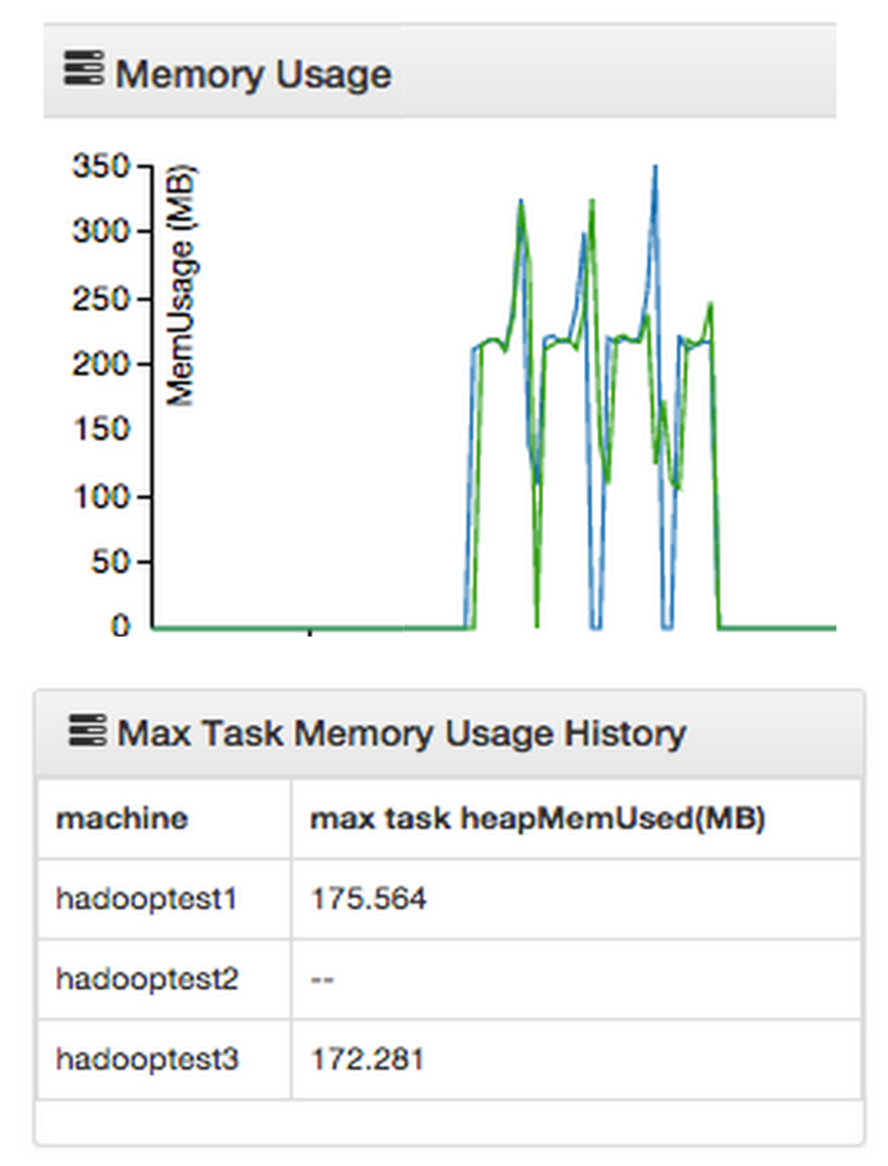
\includegraphics[width=2.1in]{image/test1a.png}
    \caption{Memory Usage under Same Threshold without Clearance}
    \label{ref:memory_allocation}
\end{figure}

In Figure 11

\begin{figure}[ht]
  \centering
    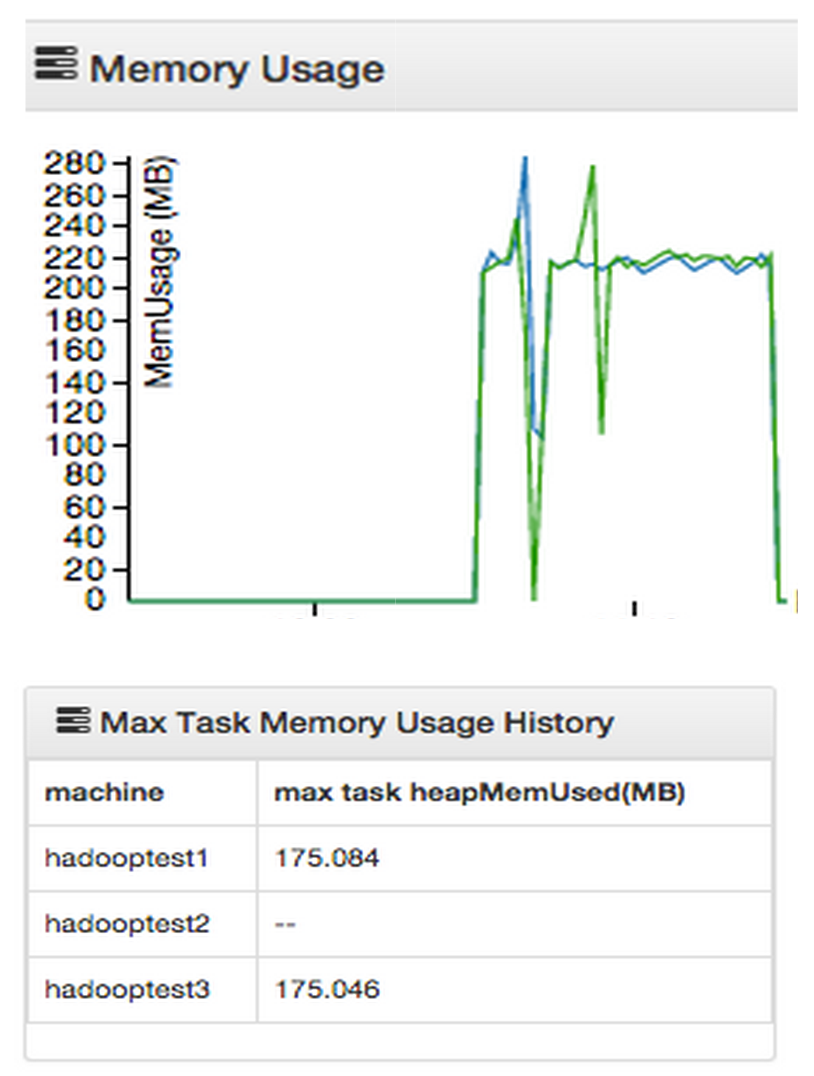
\includegraphics[width=2.1in]{image/test1b.png}
    \caption{Memory Usage under Random Threshold without Clearance}
    \label{ref:memory_allocation}
\end{figure}

\begin{figure}[ht]
  \centering
    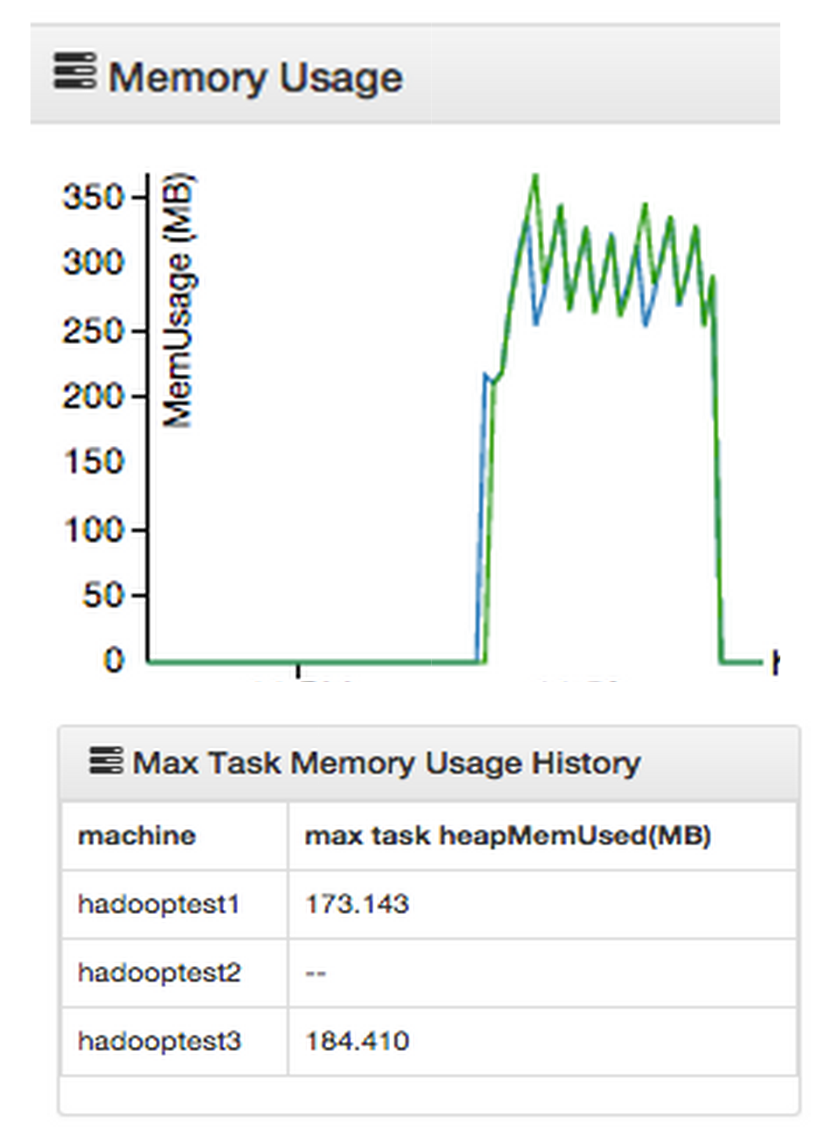
\includegraphics[width=2.1in]{image/test1c.png}
    \caption{Memory Usage under Same Threshold with Clearance}
    \label{ref:memory_allocation}
\end{figure}

\begin{figure}[ht]
  \centering
    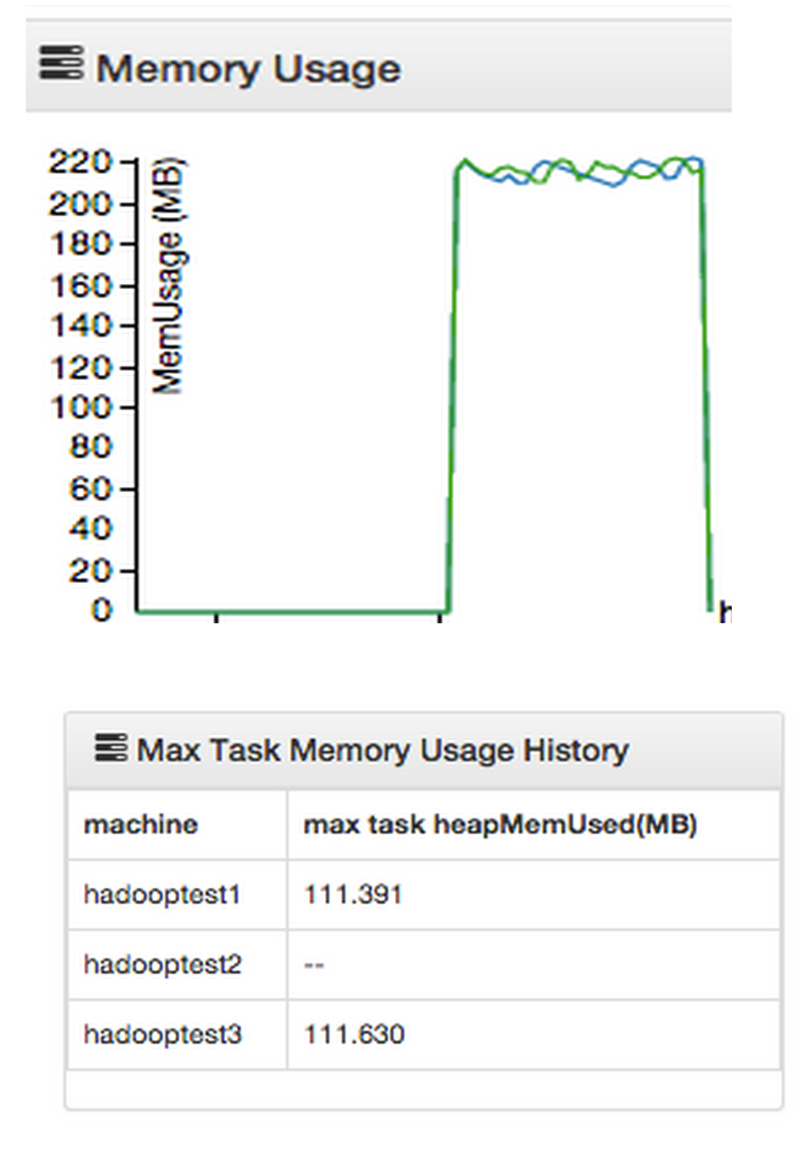
\includegraphics[width=2.1in]{image/test1d.png}
    \caption{Memory Usage under Random Threshold with Clearance}
    \label{ref:memory_allocation}
\end{figure}